\documentclass[usenames,dvipsnames]{beamer}
\usepackage{../../shared/styles/custom}
\usepackage{../../shared/styles/conventions}





\title{Conventions, Accuracy Metrics, Classification, Regression}
\date{\today}
\author{Nipun Batra and teaching staff}
\institute{IIT Gandhinagar}
\begin{document}
%% =============================================================================
% ML TEACHING MATHEMATICAL NOTATION CONVENTIONS
% =============================================================================
% Based on standard ML textbooks: Murphy's "Machine Learning: A Probabilistic Perspective",
% Bishop's "Pattern Recognition and Machine Learning", and "Mathematics for Machine Learning"

% =============================================================================
% CORE NOTATION STANDARDS
% =============================================================================

% SCALARS: Regular italics (lowercase for variables, uppercase for constants)
% Examples: x, y, n, d, k, \theta, \alpha, \lambda, \sigma

% VECTORS: Bold lowercase letters
% Examples: \mathbf{x}, \mathbf{w}, \mathbf{\mu}, \mathbf{\theta}

% MATRICES: Bold uppercase letters
% Examples: \mathbf{X}, \mathbf{W}, \mathbf{\Sigma}, \mathbf{\Lambda}

% SETS: Calligraphic uppercase
% Examples: \mathcal{D}, \mathcal{X}, \mathcal{Y}

% SPACES: Blackboard bold
% Examples: \mathbb{R}, \mathbb{Z}, \mathbb{N}

% =============================================================================
% VECTOR NOTATION (bold lowercase)
% =============================================================================

\providecommand{\vx}{\mathbf{x}}        % Input vector
\providecommand{\vy}{\mathbf{y}}        % Output vector
\providecommand{\vw}{\mathbf{w}}        % Weight vector
\providecommand{\vb}{\mathbf{b}}        % Bias vector
\providecommand{\vh}{\mathbf{h}}        % Hidden vector
\providecommand{\vz}{\mathbf{z}}        % Latent vector
\providecommand{\vf}{\mathbf{f}}        % Function vector
\providecommand{\vg}{\mathbf{g}}        % Gradient vector
\providecommand{\vu}{\mathbf{u}}        % Generic vector u
\providecommand{\vv}{\mathbf{v}}        % Generic vector v
\providecommand{\vzero}{\mathbf{0}}     % Zero vector
\providecommand{\vone}{\mathbf{1}}      % Ones vector

% Greek vectors (bold)
\providecommand{\vmu}{\boldsymbol{\mu}}     % Mean vector
\providecommand{\vtheta}{\boldsymbol{\theta}} % Parameter vector
\providecommand{\vlambda}{\boldsymbol{\lambda}} % Lambda vector
\providecommand{\valpha}{\boldsymbol{\alpha}}   % Alpha vector
\providecommand{\vbeta}{\boldsymbol{\beta}}     % Beta vector
\providecommand{\vxi}{\boldsymbol{\xi}}         % Xi vector
\providecommand{\vepsilon}{\boldsymbol{\epsilon}} % Epsilon vector

% =============================================================================
% MATRIX NOTATION (bold uppercase)
% =============================================================================

\providecommand{\mX}{\mathbf{X}}        % Data matrix
\providecommand{\mY}{\mathbf{Y}}        % Target matrix
\providecommand{\mW}{\mathbf{W}}        % Weight matrix
\providecommand{\mA}{\mathbf{A}}        % Generic matrix A
\providecommand{\mB}{\mathbf{B}}        % Generic matrix B
\providecommand{\mC}{\mathbf{C}}        % Generic matrix C
\providecommand{\mH}{\mathbf{H}}        % Hidden layer matrix / Hessian
\providecommand{\mI}{\mathbf{I}}        % Identity matrix
\providecommand{\mJ}{\mathbf{J}}        % Jacobian matrix
\providecommand{\mK}{\mathbf{K}}        % Kernel matrix
\providecommand{\mL}{\mathbf{L}}        % Loss matrix / Cholesky factor
\providecommand{\mP}{\mathbf{P}}        % Projection matrix
\providecommand{\mQ}{\mathbf{Q}}        % Orthogonal matrix
\providecommand{\mR}{\mathbf{R}}        % Rotation matrix
\providecommand{\mS}{\mathbf{S}}        % Scatter matrix
\providecommand{\mU}{\mathbf{U}}        % Left singular vectors
\providecommand{\mV}{\mathbf{V}}        % Right singular vectors

% Greek matrices (bold)
\providecommand{\mSigma}{\boldsymbol{\Sigma}}   % Covariance matrix
\providecommand{\mLambda}{\boldsymbol{\Lambda}} % Diagonal eigenvalue matrix
\providecommand{\mPhi}{\boldsymbol{\Phi}}       % Feature matrix
\providecommand{\mPsi}{\boldsymbol{\Psi}}       % Basis matrix
\providecommand{\mTheta}{\boldsymbol{\Theta}}   % Parameter matrix

% =============================================================================
% SETS AND SPACES (following Bishop/Murphy conventions)
% =============================================================================

\providecommand{\cD}{\mathcal{D}}       % Dataset
\providecommand{\cH}{\mathcal{H}}       % Hypothesis space
\providecommand{\cX}{\mathcal{X}}       % Input space
\providecommand{\cY}{\mathcal{Y}}       % Output space
\providecommand{\cF}{\mathcal{F}}       % Function space
\providecommand{\cG}{\mathcal{G}}       % Gaussian process
\providecommand{\cL}{\mathcal{L}}       % Lagrangian / Loss
\providecommand{\cN}{\mathcal{N}}       % Normal distribution
\providecommand{\cU}{\mathcal{U}}       % Uniform distribution
\providecommand{\cB}{\mathcal{B}}       % Bernoulli distribution
\providecommand{\cP}{\mathcal{P}}       % Probability distribution

% Number systems
\providecommand{\Real}{\mathbb{R}}      % Real numbers
\providecommand{\Nat}{\mathbb{N}}       % Natural numbers
\providecommand{\Int}{\mathbb{Z}}       % Integers
\providecommand{\Complex}{\mathbb{C}}   % Complex numbers

% =============================================================================
% OPERATORS AND FUNCTIONS (following standard conventions)
% =============================================================================

% Prediction notation (commonly used in ML)
\providecommand{\yhat}{\hat{\vy}}        % Predicted output vector (bold)
\providecommand{\yhati}{\hat{y}_i}       % Predicted output for sample i (scalar)

% Common ML functions (with conflict resolution)
\providecommand{\sigmoid}{}
\renewcommand{\sigmoid}{\operatorname{sigmoid}}
\providecommand{\softmax}{}
\renewcommand{\softmax}{\operatorname{softmax}}
\providecommand{\ReLU}{}
\renewcommand{\ReLU}{\operatorname{ReLU}}
\providecommand{\sign}{}
\renewcommand{\sign}{\operatorname{sign}}
\DeclareMathOperator{\Gain}{Gain}    % Information gain
\DeclareMathOperator{\Entropy}{Entropy}
% KL divergence (check for conflicts)
\providecommand{\KL}{}
\renewcommand{\KL}{\operatorname{KL}}
\DeclareMathOperator{\MSE}{MSE}      % Mean squared error
\DeclareMathOperator{\MAE}{MAE}      % Mean absolute error
\DeclareMathOperator{\RMSE}{RMSE}    % Root mean squared error

% Classification metrics (upright text)
\providecommand{\TP}{\text{TP}}          % True positives
\providecommand{\TN}{\text{TN}}          % True negatives  
\providecommand{\FP}{\text{FP}}          % False positives
\providecommand{\FN}{\text{FN}}          % False negatives
\DeclareMathOperator{\Precision}{Precision}
\DeclareMathOperator{\Recall}{Recall}
\DeclareMathOperator{\Accuracy}{Accuracy}

% Transpose and inverse
\providecommand{\tp}{^\top}             % Transpose (Bishop/Murphy style)
\providecommand{\inv}{^{-1}}            % Matrix inverse
\providecommand{\pinv}{^{\dagger}}      % Pseudoinverse

% Norms (consistent with Murphy/Bishop)
\providecommand{\norm}[1]{\|#1\|}       % Generic norm
\providecommand{\normone}[1]{\|#1\|_1}  % L1 norm
\providecommand{\normtwo}[1]{\|#1\|_2}  % L2 norm
\providecommand{\norminf}[1]{\|#1\|_\infty} % L-infinity norm
\providecommand{\normF}[1]{\|#1\|_F}    % Frobenius norm

% Optimization operators (upright as in Murphy)
\providecommand{\argmin}{}
\renewcommand{\argmin}{\operatorname*{arg\,min}}
\providecommand{\argmax}{}
\renewcommand{\argmax}{\operatorname*{arg\,max}}
\DeclareMathOperator{\minimize}{minimize}
\DeclareMathOperator{\maximize}{maximize}
\DeclareMathOperator{\subjectto}{subject\,to}

% Matrix operations (upright) - use conditional definitions
\providecommand{\tr}{}
\renewcommand{\tr}{\operatorname{tr}}       % Trace
\providecommand{\det}{}
\renewcommand{\det}{\operatorname{det}}     % Determinant
\providecommand{\rank}{}
\renewcommand{\rank}{\operatorname{rank}}   % Rank
\providecommand{\span}{}
\renewcommand{\span}{\operatorname{span}}   % Span
\providecommand{\null}{}
\renewcommand{\null}{\operatorname{null}}   % Null space
\DeclareMathOperator{\range}{range} % Range/column space
\providecommand{\diag}{}
\renewcommand{\diag}{\operatorname{diag}}   % Diagonal operator
\providecommand{\vec}{}
\renewcommand{\vec}{\operatorname{vec}}     % Vectorization operator

% Probability and statistics (Murphy/Bishop style)
\providecommand{\Prob}{\mathbb{P}}      % Probability measure
\providecommand{\Exp}{\mathbb{E}}       % Expectation
\DeclareMathOperator{\Var}{Var}     % Variance
\DeclareMathOperator{\Cov}{Cov}     % Covariance
\DeclareMathOperator{\Corr}{Corr}   % Correlation
% KL divergence already defined above
\DeclareMathOperator{\MI}{I}        % Mutual information

% Activation functions (already defined above with conflict resolution)

% =============================================================================
% STANDARD PARAMETER CONVENTIONS (Murphy/Bishop style)
% =============================================================================

% Primary parameters: θ (theta) - following Murphy's convention
% Learning rates: α, η (alpha, eta)
% Regularization: λ (lambda)
% Precision: β (beta) - following Bishop
% Variance: σ² (sigma squared)
% Standard deviation: σ (sigma)
% Mean: μ (mu)

% Common scalars:
% n - number of training examples
% d - dimensionality of input
% k - number of classes/clusters
% m - number of hidden units
% T - number of time steps
% i, j - indices

% =============================================================================
% STANDARD NOTATION EXAMPLES (Murphy/Bishop style)
% =============================================================================

% Linear regression:      y = \vw\tp\vx + b
% Matrix form:            \vy = \mX\vw + b\vone
% Logistic regression:    p(y=1|\vx) = \sigmoid(\vw\tp\vx)
% Gaussian:               \vx \sim \cN(\vmu, \mSigma)
% Parameter update:       \vtheta_{t+1} = \vtheta_t - \alpha \nabla \cL(\vtheta_t)
% Likelihood:             p(\cD|\vtheta) = \prod_{i=1}^n p(y_i|\vx_i, \vtheta)
% Posterior:              p(\vtheta|\cD) \propto p(\cD|\vtheta)p(\vtheta)
% Prediction:             p(y^*|\vx^*, \cD) = \int p(y^*|\vx^*, \vtheta)p(\vtheta|\cD)d\vtheta

% =============================================================================
% COMMON MISTAKES TO AVOID
% =============================================================================

% ❌ WRONG NOTATION          →  ✅ CORRECT NOTATION (Murphy/Bishop style)

% Transpose:
% ❌ x^t, X^t              →  ✅ \vx\tp, \mX\tp
% ❌ x', X'                →  ✅ \vx\tp, \mX\tp

% Vectors vs Matrices vs Scalars:
% ❌ X (for vector)        →  ✅ \vx (bold lowercase)
% ❌ w (for weight vector) →  ✅ \vw (bold lowercase)
% ❌ x (for data matrix)   →  ✅ \mX (bold uppercase)
% ❌ \mathbf{\theta}       →  ✅ \vtheta (Greek vectors are bold)
% ❌ \mathbf{n}            →  ✅ n (scalars are not bold)

% Sets and distributions:
% ❌ R                     →  ✅ \Real (blackboard bold for number systems)
% ❌ \mathcal{R}           →  ✅ \Real (use blackboard for reals)
% ❌ Normal               →  ✅ \cN (calligraphic for distributions)

% Functions and operators:
% ❌ argmax                →  ✅ \argmax (upright operator)
% ❌ E[X]                  →  ✅ \Exp[X] (blackboard E for expectation)
% ❌ trace(A)              →  ✅ \tr(\mA) (upright operator)

% =============================================================================
% ALGORITHM NAME CONVENTIONS
% =============================================================================

% Use standard capitalizations as in textbooks:
% k-NN, SVM, PCA, GMM, EM, MAP, ML, SGD, Adam, RMSprop
% ReLU, tanh, sigmoid, softmax

\endinput

  % Define counter for pop quizzes (only if not already defined)
  \makeatletter
  \@ifundefined{c@popquiz}{\newcounter{popquiz}}{}
  \makeatother
  \setcounter{popquiz}{0}

  \maketitle
  
  % Table of Contents
  \begin{frame}{Outline}
    \tableofcontents
  \end{frame}
  
  \section{Introduction and Demos}
  
  \begin{frame}{Demo}
	Comet browser and automation of tasks
  \end{frame}
  

 
  \begin{frame}{Revision: What is Machine Learning}
	 ``Field of study that gives computers the ability to learn
		without being explicitly programmed'' - Arthur Samuel
		[1959]

		\pause Let us work on the digit recognition problem.

		\begin{figure}[htp]
			\centering
			\begin{notebookbox}{https://nipunbatra.github.io/ml-teaching/notebooks/rule-based-vs-ml.html}
			  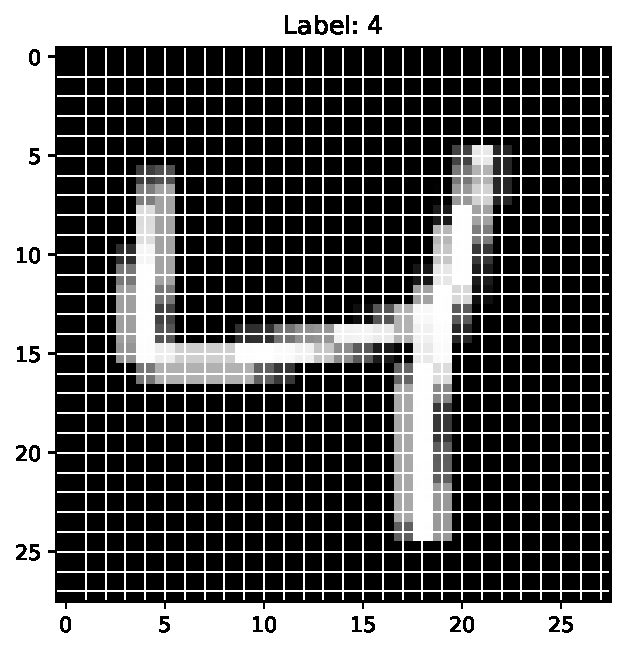
\includegraphics[scale=0.35]{../assets/accuracy-convention/figures/mnist.pdf}
			\end{notebookbox}
		  \end{figure}
		


	\end{frame}
		
	

\begin{frame}{Revision: What is Machine Learning}
	\begin{itemize}
	
	\item How would you program to recognise digits? Start with 4.
	
	\item \pause Maybe 4 can be thought of as: $\bm{|}$ + $\bm{\rule[0.5ex]{1em}{.95pt}}$ + $\bm{|}$ + another vertically down $\bm{|}$
	
	\item \pause The heights of each of the $\bm{|}$ need to be similar within tolerance
	
	\item \pause Each of the $\bm{|}$ can be slightly slanted. Similarly the horizontal line can be slanted.
	\item \pause There can be some cases of 4 where the first $\bm{|}$ is at 45 degrees
	\item \pause There can be some cases of 4 where the width of each stroke is different
	
\end{itemize}

\end{frame}	
  
 
\section{Machine Learning Fundamentals}

\begin{frame}{Traditional Programming vs Machine Learning}
\begin{center}
\begin{tikzpicture}[node distance=2cm]
  \node (D1) [startstop] {Data};
  \node (R1) [startstop, below of=D1] {Rules};
  \node (T1) [startstop, right of=D1, xshift=2cm, yshift=-1cm] {\makecell[l]{Traditional\\Programming}};
  \node (A1) [startstop, right of=T1, xshift=2cm] {Answers};
  \draw [arrow] (D1) -- (T1);
  \draw [arrow] (R1) -- (T1);
  \draw [arrow] (T1) -- (A1);
\end{tikzpicture}
\end{center}
\end{frame}


\begin{frame}{Traditional Programming}
\begin{tikzpicture}[node distance=2cm]
  \node (Data1) [startstop] {Data};
  \node (Rules1) [startstop, below of=Data1] {Rules};
  \node (Traditional) [startstop, right of=Data1, xshift=2cm, yshift=-1cm] {\makecell[l]{Traditional\\Programming}};
  \node (Answers1) [startstop, right of=Traditional, xshift=2cm] {Answers};
  \draw [arrow] (Data1) -- (Traditional);
  \draw [arrow] (Rules1) -- (Traditional);
  \draw [arrow] (Traditional) -- (Answers1);
\end{tikzpicture}
\end{frame}

\begin{frame}{Machine Learning}
\begin{tikzpicture}[node distance=2cm]
  \node (Data2) [startstop] {Data};
  \node (Answers2) [startstop, below of=Data2] {Answers};
  \node (ML) [startstop, right of=Data2, xshift=2cm, yshift=-1cm] {\makecell[l]{Machine \\Learning}};
  \node (Rules2) [startstop, right of=ML, xshift=2cm] {Rules};
  \draw [arrow] (Data2) -- (ML);
  \draw [arrow] (Answers2) -- (ML);
  \draw [arrow] (ML) -- (Rules2);
\end{tikzpicture}
\end{frame}

\begin{frame}{Revision: What is Machine Learning}
``A computer program is said to learn from
experience E with respect to some class of tasks T
and performance measure P if its performance at
tasks in T, as measured by P, improves with
experience E.'' - Tom Mitchell
\end{frame}

\begin{frame}{First ML Task: Grocery Store Tomato Quality Prediction}
Problem statement: You want to predict the quality of a tomato given its visual features.
\end{frame}

\begin{frame}{Dataset}
Imagine you have some past data on quality of tomatoes. What visual features do you think will be useful?

\begin{itemize}
	\item \pause Size
	\item \pause Colour
	\item \pause Texture
\end{itemize}
\end{frame}

\begin{frame}{Sample Dataset}
Here is our example dataset with tomato features: 

\begin{table}[]
	\begin{tabular}{|l|l|l|l||l|}
		\hline 
		\textbf{Sample} & \textbf{Colour} & \textbf{Size} & \textbf{Texture} & \textbf{Condition} \\ \hline 
		1      & Orange & Small & Smooth  & Good      \\
		2      & Red    & Small  & Rough  & Good \\
		3      & Orange & Medium & Smooth & Bad \\
		4      & Yellow & Large  & Smooth & Bad \\ \hline          
	\end{tabular}
\end{table}
\end{frame}

\section{First ML Example: Tomato Quality Prediction}

\stepcounter{popquiz}
\begin{frame}{Pop Quiz \#\thepopquiz}
\begin{popquizbox}{\thepopquiz}
Is the sample number a useful feature for predicting quality of a tomato?

\pause Answer: Usually no! Sample numbers are typically arbitrary identifiers and not meaningful features. Let us remove it.

\end{popquizbox}
\end{frame}

\begin{frame}{Pop Quiz \#\thepopquiz{} }
	\begin{popquizbox}{\thepopquiz}

When could sample number be useful?


\pause
In some cases, the sample number might be useful for tracking or auditing purposes. 
E.g. if some trucks are delayed during delivery, the sample number could help identify 
which batch of tomatoes was affected.
\end{popquizbox}

\end{frame}


\begin{frame}{Useful Features}


\pause Let us modify our data table for now.

\begin{table}[]
	\begin{tabular}{|l|l|l||l|}
		\hline 
		\textbf{Colour} & \textbf{Size} & \textbf{Texture} & \textbf{Condition} \\ \hline 
		Orange & Small & Smooth  & Good      \\
		Red    & Small  & Rough  & Good \\
		Orange & Medium & Smooth & Bad \\
		Yellow & Large  & Smooth & Bad \\ \hline 

	\end{tabular}
\end{table}
\end{frame}

\begin{frame}{Training Set}

\begin{table}[]
	\begin{tabular}{|l|l|l||l|}
		\hline 
				\rowcolor{white}
		\textbf{Colour} & \textbf{Size} & \textbf{Texture} & \textbf{Condition} \\ \hline 
		Orange & Small & Smooth  & Good      \\
		Red    & Small  & Rough  & Good \\
		Orange & Medium & Smooth & Bad \\
		Yellow & Large  & Smooth & Bad \\ \hline 
		
	\end{tabular}
\end{table}

\pause The training set consists of two parts:
\begin{enumerate}
	\item \pause \color{Lavender}{Features (Input Variables)}
	\item \pause \color{Tan}{Output or Response Variable}
\end{enumerate}
\end{frame}

\begin{frame}{Training Set}
\vspace{-5pt}
\begin{table}[]
	\begin{tabular}{|l|l|l||l|}
		\hline 
		\rowcolor{white}
		\cellcolor{Lavender}\textbf{Colour} & \cellcolor{Lavender}\textbf{Size} & \cellcolor{Lavender}\textbf{Texture} & \cellcolor{Tan}\textbf{Condition} \\ \hline 
		\cellcolor{Lavender}Orange & \cellcolor{Lavender}Small & \cellcolor{Lavender}Smooth  & \cellcolor{Tan}Good      \\
		\cellcolor{Lavender}Red    & \cellcolor{Lavender}Small  & \cellcolor{Lavender}Rough  & \cellcolor{Tan}Good \\
		\cellcolor{Lavender}Orange & \cellcolor{Lavender}Medium & \cellcolor{Lavender}Smooth & \cellcolor{Tan}Bad \\
		\cellcolor{Lavender}Yellow & \cellcolor{Lavender}Large  & \cellcolor{Lavender}Smooth & \cellcolor{Tan}Bad \\ \hline 
		
	\end{tabular}
\end{table}

\pause Computers work with numbers! We need to encode categorical data numerically (one-hot encoding):

\begin{table}[]
	\begin{tabular}{|l|l||l|l||l|l||l|}
		\hline 
		\rowcolor{white}
		\cellcolor{Lavender}\textbf{C0} & \cellcolor{Lavender}\textbf{C1} & \cellcolor{Lavender}\textbf{S0} & \cellcolor{Lavender}\textbf{S1} & \cellcolor{Lavender}\textbf{T0} & \cellcolor{Lavender}\textbf{T1} & \cellcolor{Tan}\textbf{Good?} \\ \hline 
		\cellcolor{Lavender}0 & \cellcolor{Lavender}0 & \cellcolor{Lavender}1 & \cellcolor{Lavender}0 & \cellcolor{Lavender}1 & \cellcolor{Lavender}0 & \cellcolor{Tan}1 \\
		\cellcolor{Lavender}0 & \cellcolor{Lavender}1 & \cellcolor{Lavender}1 & \cellcolor{Lavender}0 & \cellcolor{Lavender}0 & \cellcolor{Lavender}1 & \cellcolor{Tan}1 \\
		\cellcolor{Lavender}0 & \cellcolor{Lavender}0 & \cellcolor{Lavender}0 & \cellcolor{Lavender}1 & \cellcolor{Lavender}1 & \cellcolor{Lavender}0 & \cellcolor{Tan}0 \\
		\cellcolor{Lavender}1 & \cellcolor{Lavender}0 & \cellcolor{Lavender}0 & \cellcolor{Lavender}0 & \cellcolor{Lavender}1 & \cellcolor{Lavender}0 & \cellcolor{Tan}0 \\ \hline 
	\end{tabular}
\end{table}

\pause Orange=00, Red=01, Yellow=10; Small=10, Medium=01, Large=00; Smooth=10, Rough=01; Good=1, Bad=0

More details on encoding later!
\end{frame}


\begin{frame}{Data Matrix}

	\begin{table}[]
	\begin{tabular}{|l|l||l|l||l|l||l|}
		\hline 
		\rowcolor{white}
		\cellcolor{Lavender}\textbf{C0} & \cellcolor{Lavender}\textbf{C1} & \cellcolor{Lavender}\textbf{S0} & \cellcolor{Lavender}\textbf{S1} & \cellcolor{Lavender}\textbf{T0} & \cellcolor{Lavender}\textbf{T1} & \cellcolor{Tan}\textbf{Good?} \\ \hline 
		\cellcolor{Lavender}0 & \cellcolor{Lavender}0 & \cellcolor{Lavender}1 & \cellcolor{Lavender}0 & \cellcolor{Lavender}1 & \cellcolor{Lavender}0 & \cellcolor{Tan}1 \\
		\cellcolor{Lavender}0 & \cellcolor{Lavender}1 & \cellcolor{Lavender}1 & \cellcolor{Lavender}0 & \cellcolor{Lavender}0 & \cellcolor{Lavender}1 & \cellcolor{Tan}1 \\
		\cellcolor{Lavender}0 & \cellcolor{Lavender}0 & \cellcolor{Lavender}0 & \cellcolor{Lavender}1 & \cellcolor{Lavender}1 & \cellcolor{Lavender}0 & \cellcolor{Tan}0 \\
		\cellcolor{Lavender}1 & \cellcolor{Lavender}0 & \cellcolor{Lavender}0 & \cellcolor{Lavender}0 & \cellcolor{Lavender}1 & \cellcolor{Lavender}0 & \cellcolor{Tan}0 \\ \hline 
	\end{tabular}
\end{table}

\pause We call this data matrix $\mX$, and the complete dataset $\cD$:
\begin{enumerate}
	\item Feature matrix ($\mX \in \Real^{n \times d}$) containing data of $n$ samples each of which is $d$ dimensional.
	\item Output vector ($\vy \in \Real^n$) containing output variable for $n$ samples.
	\item Complete dataset: $\cD = \{(\vx_i, y_i)\}_{i=1}^n$ (set of sample-label pairs)
\end{enumerate}

\pause For this example: $n = 4$ (samples), $d = 6$ (features after one-hot encoding)

\end{frame}

\begin{frame}{Mathematical Notation Convention}
\begin{alertbox}{Mathematical Notation Convention}
Matrices use \textbf{bold uppercase} ($\mX$), vectors use \textbf{bold lowercase} ($\vy$), scalars use regular letters ($n$, $d$)
\end{alertbox}

\begin{examplebox}{Examples from Our Tomato Dataset}
\begin{itemize}
	\item \textbf{Scalars}: $n = 4$ (samples), $d = 6$ (features), $y_1 = 1$ 
	\item \pause \textbf{Vectors}: $\vy = [1, 1, 0, 0]^{\tp}$, $\vx_1 = [0, 0, 1, 0, 1, 0]^{\tp}$ 
	\item \pause \textbf{Matrices}: $\mX \in \Real^{4 \times 6}$ (feature matrix)
\end{itemize}
\end{examplebox}

\pause \textbf{Convention:} We write $[a, b, c]^{\tp}$ instead of $\begin{bmatrix} a \\ b \\ c \end{bmatrix}$ to save space
\end{frame}

\begin{frame}{Data Matrix Details}
\begin{itemize}
	\item Feature matrix: $\mX = \begin{bmatrix} \vx_1\tp \\ \vx_2\tp \\ \vdots \\ \vx_n\tp \end{bmatrix}$ where $\vx_i \in \Real^d$
	\item \pause Example: $\vx_1 = [0, 0, 1, 0, 1, 0]^{\tp}$ (Orange=00, Small=10, Smooth=10)
	\item \pause Complete dataset: $\cD = \{(\vx_i\tp, y_i)\}_{i=1}^n$
\end{itemize}

\pause For this example: $n = 4$, $d = 6$, so $\mX \in \Real^{4 \times 6}$ and $\vy \in \Real^4$
\end{frame}


\begin{frame}{Prediction Task}
Estimate condition for unseen tomatoes (\#5, 6) based on data set. 

\begin{table}[]
	\begin{tabular}{|l|l|l||l|}
		\hline 
		
		\textbf{Colour} & \textbf{Size} & \textbf{Texture} & \textbf{Condition} \\ \hline 
		Orange & Small & Smooth  & Good      \\
		Red    & Small  & Rough  & Good \\
		Orange & Medium & Smooth & Bad \\
		Yellow & Large  & Smooth & Bad \\ \hline
		Red    & Large  & Rough  & ? \\
		Orange &  Large & Rough  & ? \\ \hline          
	\end{tabular}
\end{table}
\end{frame}

\begin{frame}{Testing Set}
\textcolor{YellowGreen}{Testing set} is similar to \textcolor{Peach}{training set}, but, does not contain labels for output variable. 

\begin{table}[]
	\begin{tabular}{|l|l|l||l|}
		\hline 
		\textbf{Colour} & \textbf{Size} & \textbf{Texture} & \textbf{Condition} \\ \hline 
		\rowcolor{Peach}
		Orange & Small & Smooth  & Good      \\
		\rowcolor{Peach}
		Red    & Small  & Rough  & Good \\
		\rowcolor{Peach}
		Orange & Medium & Smooth & Bad \\
		\rowcolor{Peach}
		Yellow & Large  & Smooth & Bad \\ \hline
				\rowcolor{YellowGreen}
		Red    & Large  & Rough  & ? \\
		\rowcolor{YellowGreen}
		Orange &  Large & Rough  & ? \\ \hline          
	\end{tabular}
\end{table}
\end{frame}



\begin{frame}{Prediction Task}
We hope to:
\begin{enumerate}
	\item \pause Learn function $f$: $y = f(\vx)$ where $\vx$ represents features
	\item \pause From training dataset $\cD = \{(\vx_i, y_i)\}_{i=1}^n$
	\item \pause Predict condition for new test samples
\end{enumerate}

\pause
\begin{table}[]
	\begin{tabular}{|l|l|l||l|}
		\hline 
		\rowcolor{white}
		\cellcolor{Lavender}\textbf{Colour} & \cellcolor{Lavender}\textbf{Size} & \cellcolor{Lavender}\textbf{Texture} & \cellcolor{Tan}\textbf{Condition} \\ \hline 
		\rowcolor{Peach}
		\cellcolor{Lavender}Orange & \cellcolor{Lavender}Small & \cellcolor{Lavender}Smooth  & \cellcolor{Tan}Good      \\
		\rowcolor{Peach}
		\cellcolor{Lavender}Red    & \cellcolor{Lavender}Small  & \cellcolor{Lavender}Rough  & \cellcolor{Tan}Good \\
		\rowcolor{Peach}
		\cellcolor{Lavender}Orange & \cellcolor{Lavender}Medium & \cellcolor{Lavender}Smooth & \cellcolor{Tan}Bad \\
		\rowcolor{Peach}
		\cellcolor{Lavender}Yellow & \cellcolor{Lavender}Large  & \cellcolor{Lavender}Smooth & \cellcolor{Tan}Bad \\ \hline
		\rowcolor{YellowGreen}
		\cellcolor{Lavender}Red    & \cellcolor{Lavender}Large  & \cellcolor{Lavender}Rough  & \cellcolor{Tan}? \\
		\rowcolor{YellowGreen}
		\cellcolor{Lavender}Orange & \cellcolor{Lavender}Large & \cellcolor{Lavender}Rough  & \cellcolor{Tan}? \\ \hline          
	\end{tabular}
\end{table}

\textcolor{Peach}{\textbf{Training set}} used to learn $f$, \textcolor{YellowGreen}{\textbf{Test set}} for predictions
\end{frame}

\begin{frame}{Generalisation}
\begin{alertbox}{Key Question}
Is predicting well on our test set enough to say our model generalises?
\end{alertbox}

\pause
\begin{itemize}
	\item \textbf{Answer}: Ideally, no!
	\item \pause \textbf{Goal}: We want to predict well on \textit{all possible future inputs}
	\item \pause \textbf{Reality}: Test set is only a \textit{sample} from all possible inputs
	\item \pause \textbf{Assumption}: Test set is \textit{representative} of the true data distribution
\end{itemize}

\pause
\begin{keypointsbox}
Generalisation = Performance on \textbf{unseen data} from the same distribution as training data
\end{keypointsbox}



\end{frame}

\begin{frame}{Sample vs Population: A Simple Example}
\begin{examplebox}{Tomato Farm: 10,000 tomatoes ready for harvest}
\begin{itemize}
	\item \textbf{Population}: All 10,000 tomatoes
	\item \pause \textbf{Sample}: You inspect 100 random tomatoes  
	\item \pause \textbf{Goal}: Make decisions about all 10,000 based on your 100
\end{itemize}
\end{examplebox}

\pause
\textbf{Key Challenge:} Will your 100 tomatoes represent all 10,000? What if you only picked from one corner?

\pause
\textbf{ML Connection:} Training/test sets are samples from a larger population of all possible data
\end{frame}

\begin{frame}{From Tomatoes to Machine Learning}
\begin{figure}
	\centering
	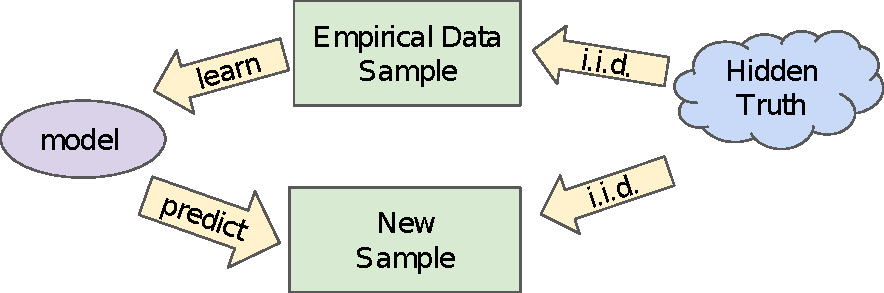
\includegraphics[width=0.7\textwidth]{../assets/accuracy-convention/diagrams/train-test.pdf}
	\caption{Image courtesy Google ML crash course}
	\label{fig:train-test}
\end{figure}

\pause \textbf{The ML Connection:}
\begin{itemize}
	\item \textbf{Population}: All possible tomato data (past, present, future)
	\item \pause \textbf{Training set}: Our 4 tomato samples (like picking from one area)
	\item \pause \textbf{Test set}: 2 new samples (like picking from another area)
\end{itemize}

\pause \textbf{Generalisation goal}: Will our model work on \textit{all future tomatoes}, not just our small samples?
\end{frame}

\begin{frame}{Second ML Task: Campus Energy Prediction}

\textbf{Regression Problem}: Predicting continuous energy consumption (kWh)

\textbf{Key factors}: \# People, Temperature

\begin{table}[]
	\begin{tabular}{|l|l||l|}
		\hline 
		\textbf{\# People} & \textbf{Temp (°C)} &  \textbf{Energy (kWh)} \\ \hline 
		4000 & 30 & 30 \\
		4200 & 30 & 32 \\
		4200 & 35 & 40 \\ \hline
		3000 & 20& ? \\
		1000 & 45 & ? \\ \hline          
	\end{tabular}
\end{table}	

\pause \textbf{Difference from tomatoes}: Energy is \textit{continuous}, not categories
\end{frame}


\begin{frame}{Classification vs Regression}
\begin{itemize}
	\item Classification
	\begin{itemize}
		\item \pause Output variable is discrete
		\item \pause i.e.  $y_i \in \{1, 2, \ldots, k\}$ where $k$ is number of classes 
		\item \pause Examples - Predicting: 
		\begin{itemize}
			\item \pause Will I get a loan? (Yes, No)
			\item \pause What is the quality of fruit? (Good, Bad)
		\end{itemize}
	\end{itemize}
	\item \pause Regression
	\begin{itemize}
		\item \pause Output variable is continuous
		\item \pause i.e.  $y_i \in \Real$ 
		\item \pause Examples - Predicting: 
		\begin{itemize}
			\item \pause How much energy will campus consume? 
			\item \pause How much rainfall will fall?
		\end{itemize}
	\end{itemize}
\end{itemize}

\end{frame}




\section{Classification vs Regression}

\stepcounter{popquiz}
\begin{frame}{Pop Quiz \#\thepopquiz}
\begin{popquizbox}{\thepopquiz}
Which of these is a regression problem?
\begin{itemize}
	\item a) Predicting if an email is spam or not
	\item b) Classifying images as cat, dog, or bird
	\item c) Predicting house prices
	\item d) Determining if a tumor is malignant or benign
\end{itemize}
\end{popquizbox}
\end{frame}

\begin{frame}{Pop Quiz \#\thepopquiz{} - Answer}
\textbf{Answer:} c) House prices are continuous values - that's regression!
\end{frame}





%\captionsetup[subtable]{labelformat=empty}
%
%\begin{frame}{Metrics for Classification}
%\begin{table}[!htb]
%	\caption{}
%	\begin{subtable}{.5\linewidth}
%		\centering
%		\caption{Prediction ($\yhat$)}
%		\begin{tabular}{ |c| } \hline 
%			
%			Good \\
%			Good \\
%			Good \\
%			Good \\
%			Bad  \\ \hline 
%			
%		\end{tabular}
%	\end{subtable}%
%	\begin{subtable}{.5\linewidth}
%		\centering
%		\caption{Ground Truth ($\vy$)}
%		\begin{tabular}{ |c| } 
%			\hline 
%			Good \\
%			Good \\
%			Bad \\
%			Bad  \\
%			Bad \\ \hline 
%		\end{tabular} \\
%	\end{subtable} 
%\end{table}
%
%\begin{align*}
%\text{Accuracy} &= \frac{||y = \hat{y}||}{||y||} \end{align*}
%\end{frame}

%\begin{frame}{Metrics for Classification}
%\begin{table}[!htb]
%	\caption{}
%	\begin{subtable}{.5\linewidth}
%		\centering
%		\caption{Prediction ($\yhat$)}
%		\begin{tabular}{ |c| } \hline 
%			
%			\rowcolor{Green}Good \\
%			\rowcolor{Green}Good \\
%			\rowcolor{Red}Good \\
%			\rowcolor{Red}Good \\
%			\rowcolor{Green}Bad  \\ \hline 
%			
%		\end{tabular}
%	\end{subtable}%
%	\begin{subtable}{.5\linewidth}
%		\centering
%		\caption{Ground Truth ($\vy$)}
%		\begin{tabular}{ |c| } 
%			\hline 
%			Good \\
%			Good \\
%			Bad \\
%			Bad  \\
%			Bad \\ \hline 
%		\end{tabular} \\
%	\end{subtable} 
%\end{table}
%
%\begin{align*}
%\text{Accuracy} &= \frac{||y = \hat{y}||}{||y||} \\
%&= \frac{3}{5} = 0.6
%\end{align*}
%\end{frame}
%
%%\begin{frame}
%%\setlength{\tabcolsep}{12pt}
%%\begin{tabular}{ cc }   % top level tables, with 2 rows
%%	Ground Truth ($\vy$) & Prediction ($\yhat$) \\  
%%	% bottom left of the top level table: table 1 
%%	\begin{tabular}{ |c| } 
%%		
%%		Good \\
%%		Good \\
%%		Good \\
%%		Good \\
%%		Bad  \\
%%		
%%	\end{tabular} &  % starting bottom right of the top level table
%%	% table 2
%%	\begin{tabular}{ |c| } 
%%		Good \\
%%		Good \\
%%		Bad \\
%%		Bad  \\
%%		Bad \\
%%	\end{tabular} \\
%%\end{tabular}
%%\end{frame}
%%
%%\begin{frame}{Metrics for Classification}
%%
%%
%%
%%$
%%Prediction (\hat{y}) = \begin{bmatrix}
%%	Good \\
%%	Good \\
%%	Good \\
%%	Good \\
%%	Bad  \\
%%\end{bmatrix} ~~~~Ground Truth (y) = \begin{bmatrix}
%%Good \\
%%Good \\
%%Bad \\
%%Bad  \\
%%Bad \\
%%\end{bmatrix}$ 
%%\vspace{30pt}
%%
%%\begin{itemize}
%%	\item Ground Truth: From the actual training set 
%%	\item Prediction: Made by the model
%%\end{itemize}
%%
%%\end{frame}
%%
%%\begin{frame}{Metrics for Classification}
%%%\DoTikzmark{num-3}{-}3 & 0 & {4}\DoTikzmark{num4}
%%$
%%Prediction (\hat{y}) = \begin{bmatrix}
%%Good \\
%%Good \\
%%Good \\
%%Good \\
%%Bad  \\
%%\end{bmatrix} ~~~~Ground Truth (y) = \begin{bmatrix}
%%Good \\
%%Good \\
%%Bad \\
%%Bad  \\
%%Bad \\
%%\end{bmatrix}$ 
%%
%%
%%\vspace{30pt}
%
%
%
%%\end{frame}


\begin{frame}{Now We Have Models - But How Good Are They?}
\begin{itemize}
	\item We've learned to predict tomato quality (classification)
	\item We've learned to predict energy consumption (regression)
	\item \pause \textbf{Key question}: How do we measure if our predictions are good?
\end{itemize}

\pause
\begin{examplebox}{The Challenge}
If our model predicts 5 tomatoes correctly and 3 incorrectly, is that good or bad? We need metrics!
\end{examplebox}

\pause
\textbf{Coming up}: Different metrics for classification vs regression problems
\end{frame}

\section{Classification Metrics}

\begin{frame}{Back to Our Tomato Example: How Did We Do?}

Let's say we trained our model and tested it on 5 new tomatoes:

\begin{table}[]
	\begin{tabular}{|c|c||c|}
		\hline 
		\textbf{\#} & \textbf{Actual} & \textbf{Predicted} \\ \hline 
		1 & Good & Good \\
		2 & Good & Good \\
		3 & Bad & Good \\
		4 & Bad & Good \\
		5 & Bad & Bad \\ \hline
	\end{tabular}
\end{table}

\pause \textbf{Questions}: 
\begin{itemize}
	\item How many did we get right? How many wrong?
	\item Is 3 out of 5 correct ``good enough''?
	\item What if getting a bad tomato wrong is worse than getting a good tomato wrong?
\end{itemize}
\end{frame}

\begin{frame}{Organizing Our Results}

Let's organize the predictions in a simpler way:

$$\bordermatrix{&\text{Model Predicted}\;(\yhat)\cr
                &\text{Good}\cr
                &\text{Good}\cr
                &\text{Good}\cr
                &\text{Good}\cr
                &\text{Bad}}
                \qquad \qquad
   \bordermatrix{&\text{Actually Was}\;(\vy)\cr
                &\text{Good}\cr
                &\text{Good}\cr
                &\text{Bad}\cr
                &\text{Bad}\cr
                &\text{Bad}}
$$

\pause \textbf{Each row} = one tomato's result

\textbf{Goal}: Create systematic ways to measure performance from these comparisons
\end{frame}

\begin{frame}{Converting to Numbers for Computation}

\textbf{Remember}: Computers work with numbers! Let's encode our categories:

\begin{examplebox}{Binary Encoding}
\textbf{Bad} = 0, \textbf{Good} = 1
\end{examplebox}

\vspace{-5pt}
Now our results become:
$$\bordermatrix{&\text{Predicted}\;(\hat{y})\cr
                &1\cr
                &1\cr
                &1\cr
                &1\cr
                &0}
                \qquad \qquad
   \bordermatrix{&\text{Ground Truth}\;(\vy)\cr
                &1\cr
                &1\cr
                &0\cr
                &0\cr
                &0}
$$

\textbf{Ground Truth} = The correct answers (what actually happened)
\end{frame}

\begin{frame}{Accuracy: Measuring Overall Performance}

\textbf{How many predictions did we get exactly right?}

$$
\bordermatrix{&\text{Predicted}\;(\yhat)\cr
               \checkmark&1\cr
               \checkmark&1\cr
                &1\cr
                &1\cr
               \checkmark&0}
\qquad \qquad
\bordermatrix{&\text{Ground Truth}\;(\vy)\cr
                &1\cr
                &1\cr
                &0\cr
                &0\cr
                &0}
$$

\pause
\begin{definitionbox}{Accuracy Formula}
$$\text{Accuracy} = \frac{\text{Number of Correct Predictions}}{\text{Total Predictions}}$$
\end{definitionbox}

\pause For our example: $\text{Accuracy} = \frac{3}{5} = 0.6$ or $60\%$

\end{frame}

\begin{frame}{Mathematical Notation: Two Ways to Count Correct Predictions}
\begin{itemize}
	\item \pause \textbf{Set cardinality notation:} $|\{i : y_i = \hat{y}_i\}|$ 
	\begin{itemize}
		\item Reads as: ``Number of indices $i$ such that $y_i = \hat{y}_i$''
		\item Counts how many samples satisfy the condition
	\end{itemize}
	
	\item \pause \textbf{Alternative: Indicator function notation}
	\begin{align*}
	\text{Accuracy} &= \frac{\sum_{i=1}^n \mathbf{1}[y_i = \hat{y}_i]}{n}
	\end{align*}
	where $\mathbf{1}[\text{condition}] = \begin{cases} 1 & \text{if condition is true} \\ 0 & \text{if condition is false} \end{cases}$
	
	\item \pause Both notations are mathematically equivalent and commonly used in ML literature
\end{itemize}

\end{frame}



\begin{frame}{Two Views: Predictions vs Confusion Matrix}

\begin{columns}[t]

\begin{column}{0.48\textwidth}
\textbf{Model Predictions}
\vspace{0.2cm}

\renewcommand{\arraystretch}{1.2}
\begin{tabular}{ccc}
\textbf{\#} & \textbf{Actual} & \textbf{Predicted} \\
\hline
1 & Good & Good \\
2 & Good & Good \\
3 & Bad & Good \\
4 & Bad & Good \\
5 & Bad & Bad \\
\end{tabular}

\end{column}

\begin{column}{0.48\textwidth}
\textbf{Confusion Matrix}
\vspace{0.2cm}

\renewcommand{\arraystretch}{1.5}
\begin{tabular}{cccc}
\multicolumn{2}{c}{} & \textbf{Bad} & \textbf{Good} \\
\multirow{2}{*}{\rotatebox[origin=c]{90}{\textbf{Pred}}} 
& \textbf{Bad} & 1 & 0 \\
& \textbf{Good} & 2 & 2 \\
\end{tabular}

\end{column}

\end{columns}

\end{frame}



\begin{frame}{Confusion Matrix: Understanding the Four Outcomes}

\begin{center}
	\renewcommand{\arraystretch}{1.5}
	\begin{tabular}{cccc}
		%\hline
		\multicolumn{2}{c}{\textbf{Confusion Matrix}} & \multicolumn{2}{c}{\textbf{Ground Truth}} \\
		%\hline
		\multicolumn{2}{c}{} & \textbf{Positive} & \textbf{Negative} \\
		%\hline
		\multirow{2}{*}{\rotatebox[origin=c]{90}{\textbf{Predicted}}} 
		& \textbf{Positive} & \cellcolor{green!40}\textbf{TP} & \cellcolor{orange!40}\textbf{FP} \\
		%\hline
		& \textbf{Negative} & \cellcolor{red!40}\textbf{FN} & \cellcolor{blue!40}\textbf{TN} \\
		%\hline
	\end{tabular}
\end{center}

\vspace{0.3cm}
\begin{definitionbox}{Four Outcomes}
	\begin{itemize}
		\item \textcolor{green!70!black}{\textbf{TP (True Positive):}} Correctly predicted positive 
		\item \textcolor{blue!70!black}{\textbf{TN (True Negative):}} Correctly predicted negative  
		\item \textcolor{orange!70!black}{\textbf{FP (False Positive):}} Wrong! Said positive but actually negative
		\item \textcolor{red!70!black}{\textbf{FN (False Negative):}} Wrong! Said negative but actually positive
	\end{itemize}
\end{definitionbox}
\end{frame}

\begin{frame}{Confusion Matrix: Precision Focus}

\begin{center}
\renewcommand{\arraystretch}{1.6}
\begin{tabular}{ccccc}
	\multicolumn{2}{c}{\textbf{Confusion Matrix}} & \multicolumn{2}{c}{\textbf{Ground Truth}} & \textbf{Row Totals} \\
	\multicolumn{2}{c}{} & \textbf{Positive} & \textbf{Negative} & \\
	\multirow{2}{*}{\rotatebox[origin=c]{90}{\textbf{Predicted}}} 
	& \textbf{Positive} & \cellcolor{green!40}TP & \cellcolor{orange!40}FP & \textbf{TP + FP} \\
	& \textbf{Negative} & FN & TN & \textbf{FN + TN} \\
	\multicolumn{2}{c}{} & \textbf{TP + FN} & \textbf{FP + TN} & \textbf{Total} \\
\end{tabular}
\end{center}

\vspace{0.4cm}
\begin{examplebox}{Focus: Predicted Positives}
$$\text{Precision} = \frac{\textcolor{green!70!black}{\textbf{TP}}}{\textcolor{green!70!black}{\textbf{TP}} + \textcolor{orange!70!black}{\textbf{FP}}}$$

``Of all predicted positives, how many were actually positive?''
\end{examplebox}

\end{frame}

\begin{frame}{Confusion Matrix: Recall Focus}

\begin{center}
\renewcommand{\arraystretch}{1.6}
\begin{tabular}{ccccc}
	\multicolumn{2}{c}{\textbf{Confusion Matrix}} & \multicolumn{2}{c}{\textbf{Ground Truth}} & \textbf{Row Totals} \\
	\multicolumn{2}{c}{} & \textbf{Positive} & \textbf{Negative} & \\
	\multirow{2}{*}{\rotatebox[origin=c]{90}{\textbf{Predicted}}} 
	& \textbf{Positive} & \cellcolor{green!40}TP & FP & \textbf{TP + FP} \\
	& \textbf{Negative} & \cellcolor{red!40}FN & TN & \textbf{FN + TN} \\
	\multicolumn{2}{c}{} & \textbf{TP + FN} & \textbf{FP + TN} & \textbf{Total} \\
\end{tabular}
\end{center}

\vspace{0.4cm}
\begin{examplebox}{Focus: Actual Positives}
$$\text{Recall} = \frac{\textcolor{green!70!black}{\textbf{TP}}}{\textcolor{green!70!black}{\textbf{TP}} + \textcolor{red!70!black}{\textbf{FN}}}$$

``Of all actual positives, how many did I catch?''
\end{examplebox}

\end{frame}

\begin{frame}{When Classes Are Imbalanced}

Many datasets have unequal class distributions!

\begin{examplebox}{Example: Medical Screening}
Out of 1000 patients tested:
\begin{itemize}
	\item \textbf{990} patients are healthy (negative class)
	\item \textbf{10} patients have the disease (positive class)
\end{itemize}
\end{examplebox}

\pause

\begin{keypointsbox}
\textbf{Why is this a problem?}
\begin{itemize}
	\item A ``lazy'' classifier that always predicts ``healthy'' gets 99\% accuracy!
	\item But it completely misses all disease cases
	\item Accuracy alone becomes misleading
\end{itemize}
\end{keypointsbox}

\pause

\textbf{Other examples:} Fraud detection, spam email, rare event prediction

\end{frame}

\begin{frame}{Cancer Detection: Comparing Two Classifiers}

\begin{columns}[t]

\begin{column}{0.48\textwidth}
\textbf{Dummy Classifier}

\vspace{0.2cm}
\scriptsize
\renewcommand{\arraystretch}{1.1}
\begin{tabular}{cccc}
	\multicolumn{2}{c}{\textbf{Confusion Matrix}} & \multicolumn{2}{c}{\textbf{Ground Truth}} \\
	\multicolumn{2}{c}{} & \textbf{Pos} & \textbf{Neg} \\
	\multirow{2}{*}{\rotatebox[origin=c]{90}{\textbf{Pred}}} 
	& \textbf{Pos} & 0 & 0 \\
	& \textbf{Neg} & 10 & 990 \\
\end{tabular}

\vspace{0.2cm}
\begin{itemize}
	\item Precision: N/A
	\item Recall: 0\%
	\item Accuracy: 99\%
\end{itemize}

\end{column}

\begin{column}{0.48\textwidth}
\textbf{Smart Classifier}

\vspace{0.2cm}
\scriptsize
\renewcommand{\arraystretch}{1.1}
\begin{tabular}{cccc}
	\multicolumn{2}{c}{\textbf{Confusion Matrix}} & \multicolumn{2}{c}{\textbf{Ground Truth}} \\
	\multicolumn{2}{c}{} & \textbf{Pos} & \textbf{Neg} \\
	\multirow{2}{*}{\rotatebox[origin=c]{90}{\textbf{Pred}}} 
	& \textbf{Pos} & 8 & 40 \\
	& \textbf{Neg} & 2 & 950 \\
\end{tabular}

\vspace{0.2cm}
\begin{itemize}
	\item Precision: \( \frac{8}{48} \approx 16.7\% \)
	\item Recall: \( \frac{8}{10} = 80\% \)
	\item Accuracy: \( \frac{8 + 950}{1000} = 95.8\% \)
\end{itemize}

\end{column}

\end{columns}

\end{frame}




\begin{frame}{Precision vs Recall: The Trade-off}


You often can't have both high precision and high recall — improving one may reduce the other.


\begin{columns}[t]
\begin{column}{0.48\textwidth}
	\begin{definitionbox}{High Precision}
	\begin{itemize}
		\item Predicts positive only when confident
		\item Low false alarms (↓ FP)
		\item May miss positives (↑ FN)
		\item Useful when FP is costly
	\end{itemize}
	\end{definitionbox}
\end{column}

\begin{column}{0.48\textwidth}
	\begin{definitionbox}{High Recall}
	\begin{itemize}
		\item Captures most positives
		\item Few misses (↓ FN)
		\item More false alarms (↑ FP)
		\item Useful when FN is costly
	\end{itemize}
	\end{definitionbox}
\end{column}
\end{columns}

\vspace{0.2cm}
\begin{examplebox}{Examples}
\textbf{Spam Filter:} Prefer precision \hfill \textbf{Cancer Test:} Prefer recall
\end{examplebox}

\end{frame}


\begin{frame}{Accuracy Metric: F1-Score}

\begin{center}
\renewcommand{\arraystretch}{1.5}
\scriptsize
\begin{tabular}{cccc}
	\multicolumn{2}{c}{\textbf{Confusion Matrix}} & \multicolumn{2}{c}{\textbf{Ground Truth}} \\
	\multicolumn{2}{c}{} & \textbf{Positive} & \textbf{Negative} \\
	\multirow{2}{*}{\rotatebox[origin=c]{90}{\textbf{Predicted}}}
	& \textbf{Positive} & \cellcolor{green!40}TP & \cellcolor{orange!40}FP \\
	& \textbf{Negative} & \cellcolor{red!40}FN & \cellcolor{blue!40}TN \\
\end{tabular}
\end{center}

\vspace{0.4cm}
\begin{examplebox}{F1-Score: Balancing Precision and Recall}
\[
\text{F1} = \frac{2 \times \text{Precision} \times \text{Recall}}{\text{Precision} + \text{Recall}}
\]
\end{examplebox}

\end{frame}

\begin{frame}{Accuracy Metric: Matthews Correlation Coefficient (MCC)}

\begin{center}
\renewcommand{\arraystretch}{1.5}
\scriptsize
\begin{tabular}{cccc}
	\multicolumn{2}{c}{\textbf{Confusion Matrix}} & \multicolumn{2}{c}{\textbf{Ground Truth}} \\
	\multicolumn{2}{c}{} & \textbf{Positive} & \textbf{Negative} \\
	\multirow{2}{*}{\rotatebox[origin=c]{90}{\textbf{Predicted}}}
	& \textbf{Positive} & \cellcolor{green!40}TP & \cellcolor{orange!40}FP \\
	& \textbf{Negative} & \cellcolor{red!40}FN & \cellcolor{blue!40}TN \\
\end{tabular}
\end{center}

\vspace{0.4cm}
\begin{examplebox}{MCC: Balanced Performance Measure}
\[
\text{MCC} = \frac{TP \cdot TN - FP \cdot FN}{\sqrt{(TP+FP)(TP+FN)(TN+FP)(TN+FN)}}
\]
\end{examplebox}

\end{frame}

\begin{frame}{MCC Comparison: Dummy vs Smart Classifier}

\begin{columns}[t]

\begin{column}{0.48\textwidth}
\textbf{Dummy Classifier}

\vspace{0.2cm}
\scriptsize
\renewcommand{\arraystretch}{1.1}
\begin{tabular}{cccc}
	\multicolumn{2}{c}{Confusion Matrix} & \multicolumn{2}{c}{Ground Truth} \\
	\multicolumn{2}{c}{} & Pos & Neg \\
	\multirow{2}{*}{\rotatebox[origin=c]{90}{Pred}} 
	& Pos & 0 & 0 \\
	& Neg & 10 & 990 \\
\end{tabular}

\vspace{0.3cm}
\[
\text{MCC} = 0 \quad \text{(denominator undefined; treat as 0)}
\]

\end{column}

\begin{column}{0.48\textwidth}
\textbf{Smart Classifier}

\vspace{0.2cm}
\scriptsize
\renewcommand{\arraystretch}{1.1}
\begin{tabular}{cccc}
	\multicolumn{2}{c}{Confusion Matrix} & \multicolumn{2}{c}{Ground Truth} \\
	\multicolumn{2}{c}{} & Pos & Neg \\
	\multirow{2}{*}{\rotatebox[origin=c]{90}{Pred}} 
	& Pos & 8 & 40 \\
	& Neg & 2 & 950 \\
\end{tabular}

\vspace{0.3cm}
\[
\text{MCC} = 
\frac{7600}{\sqrt{(48)(10)(990)(952)}} \approx \textbf{0.26}
\]

\end{column}

\end{columns}

\end{frame}



% \begin{frame}{Precision: Focus on Predicted Positives}

% \textbf{When we predict ``Good'', how often are we correct?}

% $$
% \bordermatrix{&\text{Predicted}\;(\yhat)\cr
%                \rightarrow\checkmark&\text{Good}\cr
%                \rightarrow\checkmark&\text{Good}\cr
%                 \rightarrow&\text{Good}\cr
%                 \rightarrow&\text{Good}\cr
%                &\text{Bad}}
% \qquad \qquad
% \bordermatrix{&\text{Ground Truth}\;(\vy)\cr
%                 &\text{Good}\cr
%                 &\text{Good}\cr
%                 &\text{Bad}\cr
%                 &\text{Bad}\cr
%                 &\text{Good}}
% $$

% \pause
% \begin{definitionbox}{Precision Formula}
% $$\text{Precision} = \frac{\text{Correct Positive Predictions}}{\text{All Positive Predictions}} = \frac{\textcolor{green!70!black}{\textbf{TP}}}{\textcolor{green!70!black}{\textbf{TP}} + \textcolor{orange!70!black}{\textbf{FP}}}$$
% \end{definitionbox}

% \pause For our example: $\text{Precision} = \frac{2}{4} = 0.5$ or $50\%$

% \textbf{Interpretation:} Half of our ``Good'' predictions were actually correct

% \end{frame}

% \begin{frame}{Recall: Focus on Actual Positives}

% \textbf{Of all the ``Good'' tomatoes, how many did we correctly identify?}

% $$
% \bordermatrix{&\text{Predicted}\;(\yhat)\cr
%                \rightarrow\checkmark&\text{Good}\cr
%                \rightarrow\checkmark&\text{Good}\cr
%                 &\text{Good}\cr
%                 &\text{Good}\cr
%                \rightarrow&\text{Bad}}
% \qquad \qquad
% \bordermatrix{&\text{Ground Truth}\;(\vy)\cr
%                 \rightarrow&\text{Good}\cr
%                 \rightarrow&\text{Good}\cr
%                 &\text{Bad}\cr
%                 &\text{Bad}\cr
%                 \rightarrow&\text{Good}}
% $$

% \pause
% \begin{definitionbox}{Recall Formula}
% $$\text{Recall} = \frac{\text{Correct Positive Predictions}}{\text{All Actual Positives}} = \frac{\textcolor{green!70!black}{\textbf{TP}}}{\textcolor{green!70!black}{\textbf{TP}} + \textcolor{red!70!black}{\textbf{FN}}}$$
% \end{definitionbox}

% \pause For our example: $\text{Recall} = \frac{2}{3} = 0.67$ or $67\%$

% \textbf{Interpretation:} We correctly identified $67\%$ of all actually good tomatoes

% \end{frame}

% \stepcounter{popquiz}
% \begin{frame}{Pop Quiz \#\thepopquiz}
% \begin{popquizbox}{\thepopquiz}
% In a dataset of 1000 samples where only 10 are positive cases, what's the accuracy of a classifier that always predicts "negative"?
% \begin{itemize}
% 	\item a) 1\%
% 	\item b) 50\% 
% 	\item c) 90\%
% 	\item d) 99\%
% \end{itemize}
% \end{popquizbox}
% \end{frame}

% \begin{frame}{Pop Quiz \#\thepopquiz{} - Answer}
% \textbf{Answer:} d) 99\% - but this classifier is useless! This shows why accuracy can be misleading.
% \end{frame}

% \begin{frame}{Real-World Example: Cancer Detection}
% Given predictions of whether a tissue is cancerous or not ($n = 100$).
% $$
% \bordermatrix{&\text{Predicted}\;(\yhat)\cr
%                \rightarrow&\text{Yes}\cr
%                &\text{No}\cr
%                 &\text{No}\cr
%                 &\ldots\cr
%                &\text{No}}
% \qquad \qquad
% \bordermatrix{&\text{Ground Truth}\;(\vy)\cr
%                 &\text{No}\cr
%                 &\text{No}\cr
%                 &\ldots\cr
%                 &\text{No}\cr
%                 \rightarrow&\text{Yes}}
%             $$

% \pause 
% \begin{alertbox}{Problem with Accuracy Alone}
% \begin{align*}
% \text{Accuracy} = \frac{98}{100} = 98\% \qquad \text{Recall} = \frac{0}{1} = 0\% \qquad \text{Precision} = \frac{0}{1} = 0\%
% \end{align*}
% \textbf{98\% accuracy sounds great, but we missed the only cancer case!}
% \end{alertbox}

% \end{frame}



% \begin{frame}{Accuracy Metrics: Example}
% For the data given below, calculate: 
% $$
% \bordermatrix{&\text{G.T. Positive}&\text{G.T. Negative}\cr
%                \text{Pred Positive}&90&4\cr
%                \text{Pred Negative}&1&1}
% $$

% Precision = ?  \\
% Recall = ?\\
% F-Score = ?\\
% Matthew's Coeff. = ?\\
% \end{frame}

% \begin{frame}{Accuracy Metrics: Answer}
% For the same data
% $$
% \bordermatrix{&\text{G.T. Positive}&\text{G.T. Negative}\cr
%                \text{Pred Positive}&90&4\cr
%                \text{Pred Negative}&1&1}
% $$

% Precision = $\frac{90}{94}$ \\
% Recall = $\frac{90}{91}$ \\
% F-Score = 0.9524 \\
% Matthew's Coeff. = 0.14
% \end{frame}




\begin{frame}{Confusion Matrix for multi-class classification}
	\begin{figure}[htp]
		\centering
		\begin{notebookbox}{https://nipunbatra.github.io/ml-teaching/notebooks/confusion-mnist.html}
		  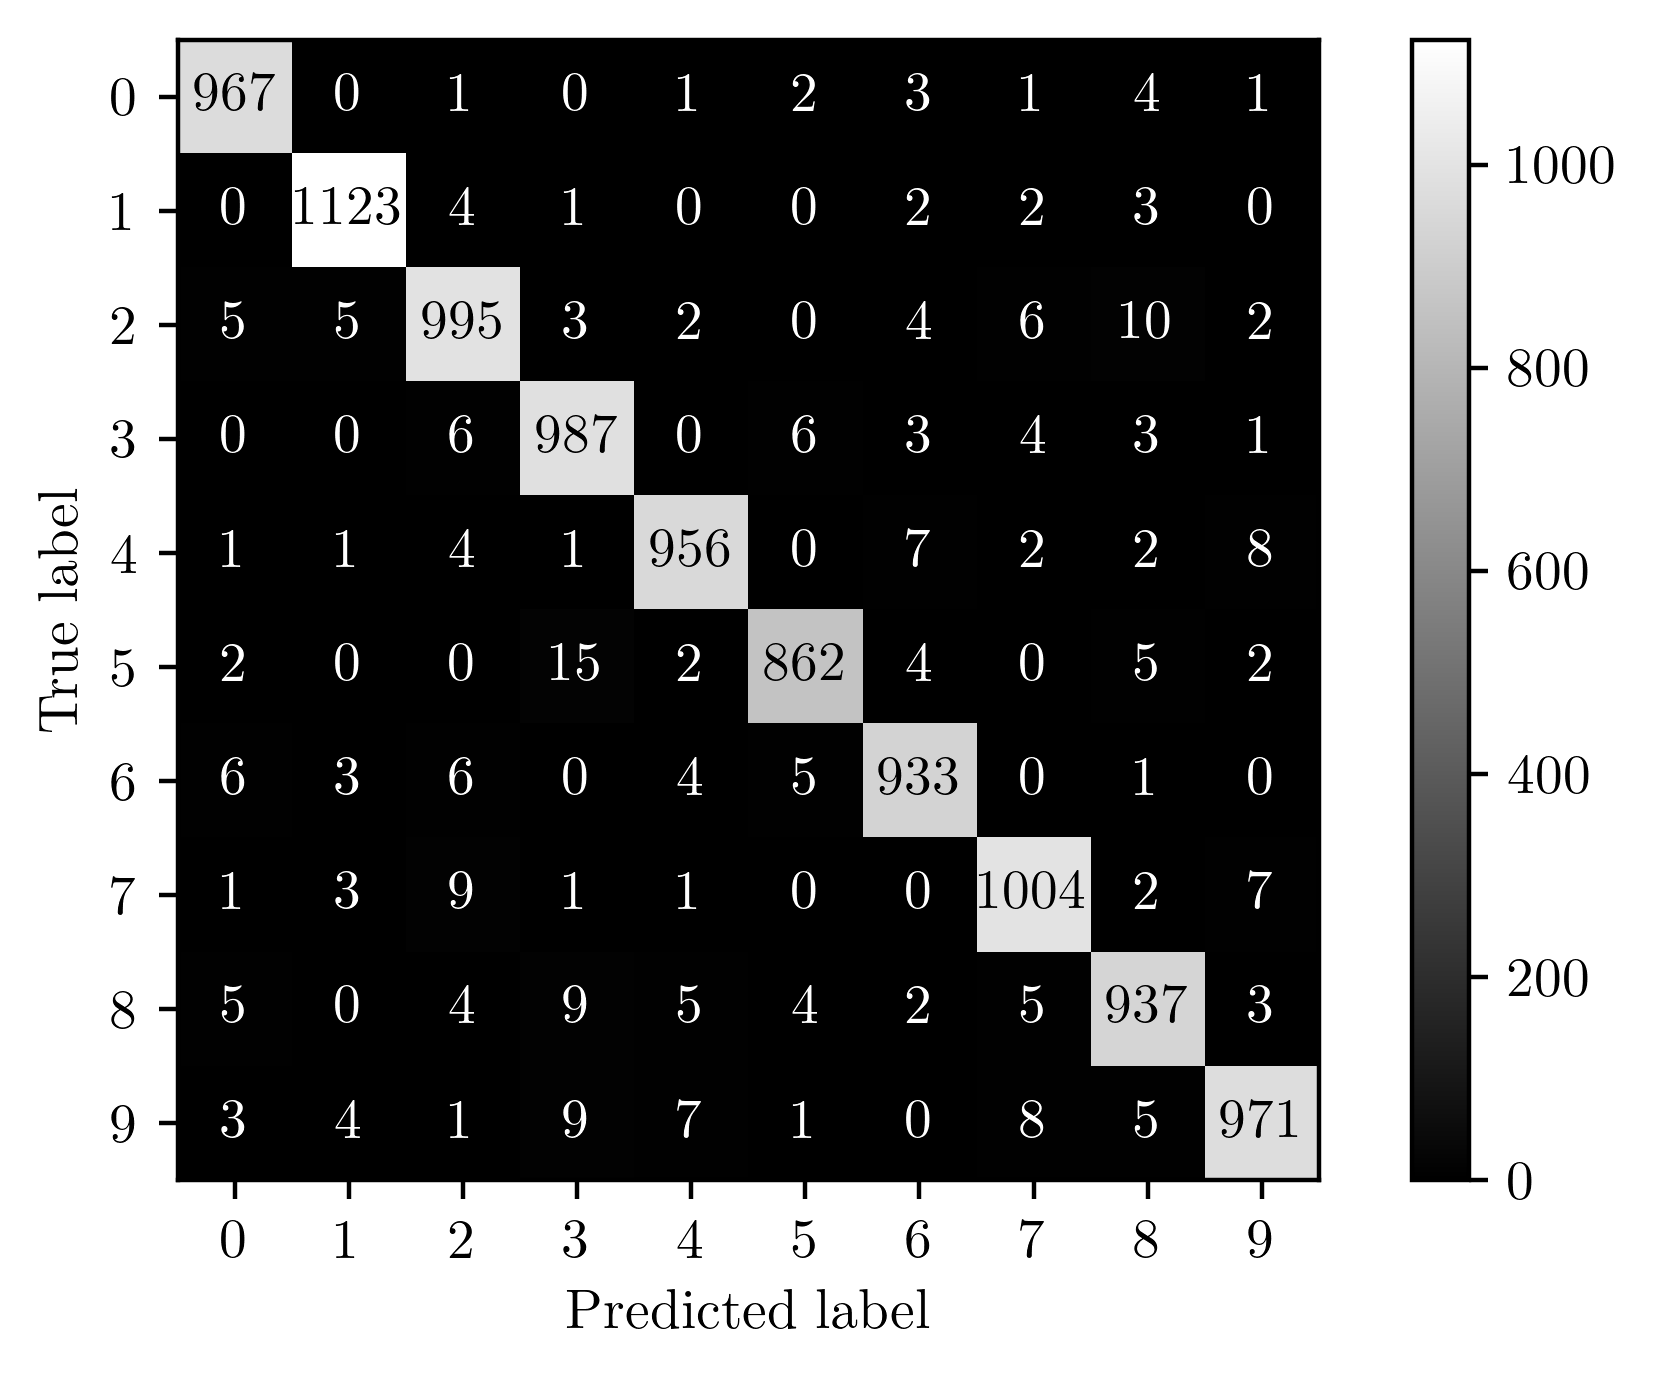
\includegraphics[scale=0.5]{../assets/accuracy-convention/figures/mnist-cm.png}
		\end{notebookbox}
	  \end{figure}
	
\end{frame}



\section{Regression Metrics}

\begin{frame}{Metrics for Regression: MSE \& MAE}
$$
\bordermatrix{&\text{Prediction}\;(\hat{y})\cr
               &10\cr
               &20\cr
                &30\cr
                &40\cr
               &50}
\qquad \qquad
\bordermatrix{&\text{Ground Truth}\;(\vy)\cr
               &20\cr
               &30\cr
                &40\cr
                &50\cr
               &60}
$$

\begin{align*}
\text{\textcolor{red}{Mean} \textcolor{green}{Squared} \textcolor{Tan}{Error} (MSE)} &=  \frac{\mathcolor{red}{\sum_{i=1}^{n}}(\mathcolor{Tan}{\hat{y}_i-y_i)}^{\mathcolor{green}2}}{\mathcolor{red}{n}} \\ 
\text{Root Mean Square Error (RMSE)} &=  \sqrt{\text{MSE}}
\end{align*}

\end{frame}

\begin{frame}{Accuracy Metrics: MAE \& ME}
$$
\bordermatrix{&\text{Prediction}\;(\hat{y})\cr
               &10\cr
               &20\cr
                &30\cr
                &40\cr
               &50}
\qquad \qquad
\bordermatrix{&\text{Ground Truth}\cr
               &20\cr
               &30\cr
                &40\cr
                &50\cr
               &60}
$$

\begin{align*}
\text{\textcolor{red}{Mean} \textcolor{green}{Absolute} \textcolor{Tan}{Error} (MAE)} &=  \frac{\mathcolor{red}{\sum_{i=1}^{n}}\mathcolor{green}|\mathcolor{Tan}{\hat{y}_i-y_i\mathcolor{green}|}}{\mathcolor{red}{n}} \\ 
\text{Mean Error} &=  \frac{\sum_{i=1}^{n}(\hat{y}_i-y_i)}{n}
\end{align*}
\pause Is there any downside with using mean error?\\
\pause Errors can get cancelled out

\end{frame}

% \stepcounter{popquiz}
% \begin{frame}{Pop Quiz \#\thepopquiz}
% \begin{popquizbox}{\thepopquiz}
% Why might Mean Absolute Error (MAE) be preferred over Mean Squared Error (MSE)?
% \begin{itemize}
% 	\item a) MAE is always smaller
% 	\item b) MAE is less sensitive to outliers
% 	\item c) MAE is easier to compute
% 	\item d) MAE works only for classification
% \end{itemize}
% \end{popquizbox}
% \end{frame}

% \begin{frame}{Pop Quiz \#\thepopquiz{} - Answer}
% \textbf{Answer:} b) MAE is less sensitive to outliers since it doesn't square the errors!
% \end{frame}



\section{Data Visualization and Baselines}

\begin{frame}{The Importance of Plotting}
    \begin{figure}[htp]
      \centering
      \begin{notebookbox}{https://nipunbatra.github.io/ml-teaching/notebooks/anscombe.html}
        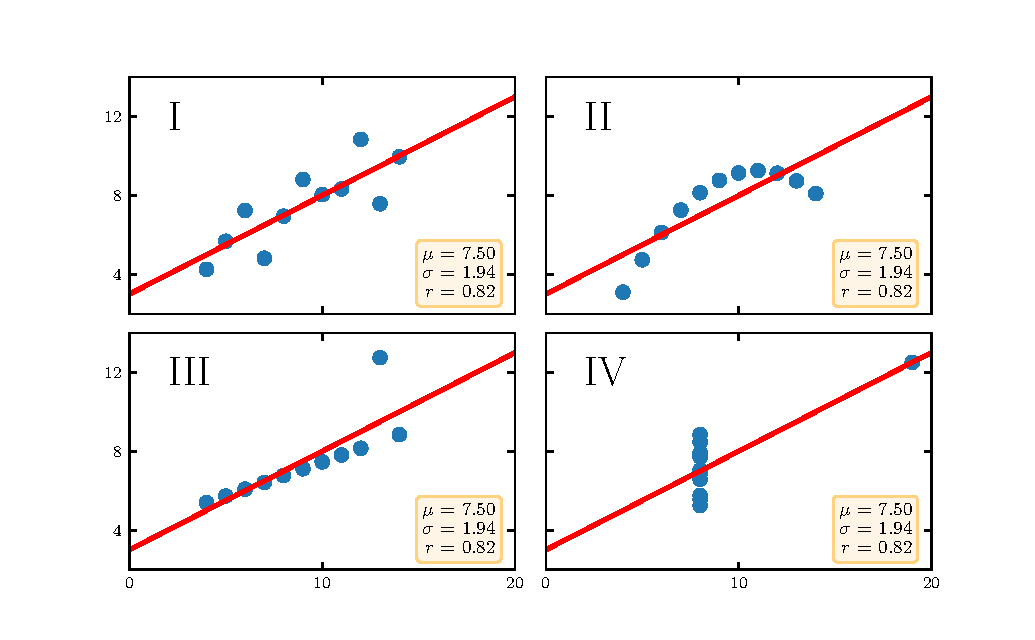
\includegraphics[width=\linewidth]{../assets/accuracy-convention/figures/anscombe.pdf}
      \end{notebookbox}
      \caption{Anscombe’s Quartet}
    \end{figure}
  \end{frame}

  \begin{frame}{Dummy Baselines}
	\begin{notebookbox}{https://nipunbatra.github.io/ml-teaching/notebooks/dummy-baselines.html}
	  \end{notebookbox}
\end{frame}

\begin{frame}{The Importance of Plotting}
\begin{tabular}{|c|c|c|}
\hline 
Property & Value & Across datasets \\ 
\hline 
mean(X) & 9 & exact \\ 
mean(Y) & 7.5 & up to 3 decimal places \\ 
Linear regression line & 	y = 3.00 + 0.500x & up to 2 decimal places \\ 
\hline 
\end{tabular} 


\end{frame}

\section{Summary and Key Takeaways}

\stepcounter{popquiz}
\begin{frame}{Pop Quiz \#\thepopquiz}
\begin{popquizbox}{\thepopquiz}
For imbalanced datasets, which metrics should you prioritize over accuracy?
\begin{itemize}
	\item a) Only precision
	\item b) Only recall
	\item c) Precision, recall, and F1-score
	\item d) Only confusion matrix
\end{itemize}
\end{popquizbox}
\end{frame}

\begin{frame}{Pop Quiz \#\thepopquiz{} - Answer}
\textbf{Answer:} c) Precision, recall, and F1-score give a more complete picture!
\end{frame}

\begin{frame}{Key Takeaways}
\begin{keypointsbox}
\begin{itemize}
	\item \textbf{ML vs Traditional Programming:} ML learns rules from data, traditional programming uses predefined rules
	\item \textbf{Features matter:} Choose meaningful features, avoid arbitrary identifiers
	\item \textbf{Classification vs Regression:} Discrete outputs vs continuous outputs
	\item \textbf{Accuracy isn't everything:} For imbalanced data, use precision, recall, F1-score
	\item \textbf{Visualization is crucial:} Always plot your data (Anscombe's Quartet lesson)
	\item \textbf{Use baselines:} Simple baseline models help validate your approach
\end{itemize}
\end{keypointsbox}
\end{frame}

% \begin{frame}{Summary: Evaluation Metrics}

% \scriptsize
% \begin{center}
% \renewcommand{\arraystretch}{1.3}
% \begin{tabular}{|p{2.8cm}|p{3.2cm}|p{4.5cm}|}
% \hline
% \textbf{Task} & \textbf{Common Metrics} & \textbf{When to Use} \\
% \hline
% Classification & Accuracy, Precision, Recall, F1, Confusion Matrix & 
% - Balanced vs. imbalanced data \newline
% - Multi-class settings \\
% \hline
% Regression & MSE, RMSE, MAE, Mean Error & 
% - Continuous output \newline
% - Check for bias and variance \\
% \hline
% \end{tabular}
% \end{center}

% \vspace{0.6cm}
% \textbf{Reminder:} \textit{Pick metrics that align with your problem and what matters in practice.}

% \end{frame}



\end{document}
